%%%%%%%%%%%%%%%%%%%%%%%%%%%%%%%%%%%%%%%%%
% Short Sectioned Assignment
% LaTeX Template
% Version 1.0 (5/5/12)
%
% This template has been downloaded from:
% http://www.LaTeXTemplates.com
%
% Original author:
% Frits Wenneker (http://www.howtotex.com)
%
% License:
% CC BY-NC-SA 3.0 (http://creativecommons.org/licenses/by-nc-sa/3.0/)
%
%%%%%%%%%%%%%%%%%%%%%%%%%%%%%%%%%%%%%%%%%

%----------------------------------------------------------------------------------------
%	PACKAGES AND OTHER DOCUMENT CONFIGURATIONS
%----------------------------------------------------------------------------------------

\documentclass[paper=a4, fontsize=11pt]{scrartcl} % A4 paper and 11pt font size

\usepackage[T1]{fontenc} % Use 8-bit encoding that has 256 glyphs
\usepackage{fourier} % Use the Adobe Utopia font for the document - comment this line to return to the LaTeX default
\usepackage[english]{babel} % English language/hyphenation
\usepackage{amsmath,amsfonts,amsthm} % Math packages

\usepackage{graphicx}

\usepackage{sectsty} % Allows customizing section commands
\allsectionsfont{\centering \normalfont\scshape} % Make all sections centered, the default font and small caps

\usepackage[procnames]{listings}

\usepackage{fancyhdr} % Custom headers and footers
\pagestyle{fancyplain} % Makes all pages in the document conform to the custom headers and footers
\fancyhead{} % No page header - if you want one, create it in the same way as the footers below
\fancyfoot[L]{} % Empty left footer
\fancyfoot[C]{} % Empty center footer
\fancyfoot[R]{\thepage} % Page numbering for right footer
\renewcommand{\headrulewidth}{0pt} % Remove header underlines
\renewcommand{\footrulewidth}{0pt} % Remove footer underlines
\setlength{\headheight}{13.6pt} % Customize the height of the header

\numberwithin{equation}{section} % Number equations within sections (i.e. 1.1, 1.2, 2.1, 2.2 instead of 1, 2, 3, 4)
\numberwithin{figure}{section} % Number figures within sections (i.e. 1.1, 1.2, 2.1, 2.2 instead of 1, 2, 3, 4)
\numberwithin{table}{section} % Number tables within sections (i.e. 1.1, 1.2, 2.1, 2.2 instead of 1, 2, 3, 4)

\setlength\parindent{0pt} % Removes all indentation from paragraphs - comment this line for an assignment with lots of text

%----------------------------------------------------------------------------------------
%	TITLE SECTION
%----------------------------------------------------------------------------------------

\newcommand{\horrule}[1]{\rule{\linewidth}{#1}} % Create horizontal rule command with 1 argument of height

\title{	
\normalfont \normalsize 
\textsc{BRSU} \\ [25pt] % Your university, school and/or department name(s)
\horrule{0.5pt} \\[0.4cm] % Thin top horizontal rule
\huge Neural Networks\\Assignment 7 \\ % The assignment title
\horrule{2pt} \\[0.5cm] % Thick bottom horizontal rule
}

\author{Bastian Lang} % Your name

\date{\normalsize\today} % Today's date or a custom date

\begin{document}

\maketitle % Print the title

\newpage

\section{Outline}

\begin{itemize}
	\item Output Representation and Decision Rule
	
	\item Computer Experiment
	\begin{itemize}
		\item Bayesian Decision Boundary
		\item Experimental Determination of Optimal Multilayer Perceptron
		\begin{itemize}
			\item Optimal Number of Hidden Neurons
			\item Optimal Learning and Momentum Constants
			\item Evaluation of Optimal Network Design
		\end{itemize}
	\end{itemize}
	
	\item Feature Detection
	\begin{itemize}
		\item Relation to Fisher's Linear Discriminent
	\end{itemize}
	
	\item Back-Propagation and Differentation
	\begin{itemize}
		\item Jacobian Matrix
	\end{itemize}
	
	\item Hessian Matrix
	
	\item Generalization
	\begin{itemize}
		\item Sufficient Training Set Size for a Valid Generalization
	\end{itemize}
	
	\item Approximation of Functions
	\begin{itemize}
		\item Universal Approximation Theorem
		\item Bounds on Approximation Errors
		\item Curse of Dimensionality
		\item Practical Considerations
	\end{itemize}
	
	\item Cross-Validation
	\begin{itemize}
		\item Model Selection
		\item Early Stopping Method of Training
		\item Variants of Cross-Validation
	\end{itemize}
	
	\item Network Pruning Techniques
	\begin{itemize}
		\item Complexity-Regularization
		\item Weight Decay
		\item Weight Elimination
		\item Approximate Smoother
		\item Hessian-based Network Pruning
		\item Computing the inverse Hessian matrix
	\end{itemize}
	
	\item Virtues and Limitations of Back-Propagation Learning
	\begin{itemize}
		\item Connectionism
		\item Feature Detection
		\item Function Approximation
		\item Computational Efficiency
		\item Sensitivity Analysis
		\item Robustness
		\item Convergence
		\item Local Minima
		\item Scaling
	\end{itemize}
	
	\item Accelerated Convergence of Back-Propagation Learning
	\begin{itemize}
		\item 4 Heuristics
	\end{itemize}
	
	\item Supervised Learning viewed as an Optimization Problem
	\begin{itemize}
		\item Conjugate-Gradient Method
		\item Example
		\item Summary of the Nonlinear Conjugate Gradient Algorithm
		\item Quasi-Newton Methods
		\item Comparison of Quasi-Newton Methods with Conjugate-Gradient Methods
	\end{itemize}
	
	\item Convolutional Networks
	
	
	\item Summary and Discussion
\end{itemize}

\section{PCA \& ICA}

\subsection{output}
\begin{figure}[ht]
	\centering
  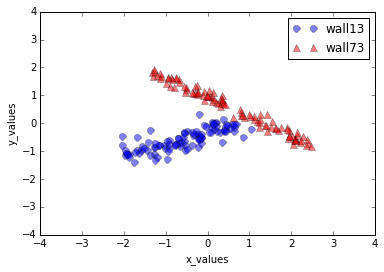
\includegraphics[width=0.8\textwidth]{combined.png}
	\caption{Both datasets in new coordinate system after performing PCA.}
	\label{fig1}
\end{figure}

\begin{figure}[ht]
	\centering
  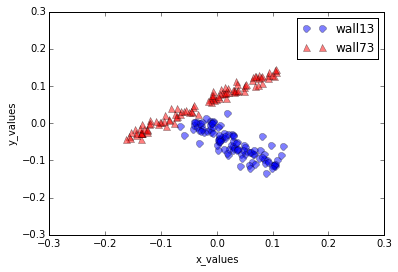
\includegraphics[width=0.8\textwidth]{combined_ica.png}
	\caption{Both datasets in new coordinate system after performing ICA.}
	\label{fig1}
\end{figure}

\subsection{code}
\begin{lstlisting}
# -*- coding: utf-8 -*-
"""
Created on Sat Nov 21 12:41:57 2015

@author: bastian
"""

from matplotlib.mlab import PCA as mlabPCA
import matplotlib.pyplot as plt
import numpy as np
from sklearn.decomposition import FastICA as ICA
from sklearn.cluster import KMeans
import neurolab as nl


def cluster_data(data,class_label):
    
    result = KMeans(n_clusters=2, random_state=170).fit_predict(data)
    

    plt.scatter(data[:,0],data[:,1], c=result)

    plt.xlabel('x_values')
    plt.ylabel('y_values')
    plt.xlim([-4,4])
    plt.ylim([-4,4])
    plt.legend()
    plt.title('Transformed samples versus original data')
    
    plt.show()


def do_ica(data, class_label):
    
    # ica
    ica = ICA()
    result = ica.fit(data).transform(data)
    
    

    plt.plot(result[:,0],result[:,1],
             'o', markersize=7, color='blue', alpha=0.5, label=class_label)

    plt.xlabel('x_values')
    plt.ylabel('y_values')
    plt.xlim([-0.5,0.5])
    plt.ylim([-0.5,0.5])
    plt.legend()
    plt.title('Transformed samples versus original data')
    
    plt.show()
    

def do_pca(data, class_label):
    
    mlab_pca = mlabPCA(wall13_data)
    
    
    print('PC axes in terms of the measurement axes scaled by the standard deviations:\n', mlab_pca.Wt)
    
    # pca
    plt.plot(mlab_pca.Y[:,0],mlab_pca.Y[:,1],
             'o', markersize=7, color='blue', alpha=0.5, label=class_label)
    # original
    plt.plot(wall13_data[:,0], wall13_data[:,1],'^', markersize=7, color='red', alpha=0.5, label='original')
    
    plt.xlabel('x_values')
    plt.ylabel('y_values')
    plt.xlim([-4,40])
    plt.ylim([-4,10])
    plt.legend()
    plt.title('Transformed samples versus original data')
    
    plt.show()
    
    return mlab_pca.Y



def split_pca(combined_data, label_1, label_2):
    
    mlab_pca = mlabPCA(combined_data)
    
    print('PC axes in terms of the measurement axes scaled by the standard deviations:\n', mlab_pca.Wt)
    
    plt.plot(mlab_pca.Y[0:100,0],mlab_pca.Y[0:100,1],
             'o', markersize=7, color='blue', alpha=0.5, label=label_1)
    plt.plot(mlab_pca.Y[100:200,0], mlab_pca.Y[100:200,1],
             '^', markersize=7, color='red', alpha=0.5, label=label_2)
    
    plt.xlabel('x_values')
    plt.ylabel('y_values')
    plt.xlim([-4,4])
    plt.ylim([-4,4])
    plt.legend()
    #plt.title('Transformed samples with class labels from matplotlib.mlab.PCA()')
    
    plt.show()
    
    return mlab_pca.Y
   

def split_ica(combined_data, label_1, label_2):
    
    ica = ICA()
    result = ica.fit(combined_data).transform(combined_data)
    
    
    plt.plot(result[0:100,0],result[0:100,1],
             'o', markersize=7, color='blue', alpha=0.5, label=label_1)
    plt.plot(result[100:200,0], result[100:200,1],
             '^', markersize=7, color='red', alpha=0.5, label=label_2)
    
    plt.xlabel('x_values')
    plt.ylabel('y_values')
    plt.xlim([-0.3,0.3])
    plt.ylim([-0.3,0.3])
    plt.legend()
    #plt.title('Transformed samples with class labels from matplotlib.mlab.PCA()')
    
    plt.show()
    
    return result

wall13_data = np.genfromtxt('wall13.csv', delimiter=',')
do_pca(wall13_data, 'wall13')
#o_ica(wall13_data, 'wall13')   


wall73_data = np.genfromtxt('wall73.csv', delimiter=',')
do_pca(wall73_data, 'wall73')
do_ica(wall73_data, 'wall73')    

mixed_data = np.concatenate((wall13_data, wall73_data), axis=0)
Y = split_pca(mixed_data, 'wall13', 'wall73')
split_ica(mixed_data, 'wall13', 'wall73')
#cluster_data(Y, 'mixed')
\end{lstlisting}



\end{document}